\section{Reproduction Results}\label{sec:repro}

The target is the gap between HippoRAG~2 and dense retrieval with the same embedder, not the paper's absolute numbers.
Both systems index all 11,656 passages; evaluation uses the first $N$ questions of the released 1,000-question sample.
Dense retrieval ranks with HippoRAG's own passage vectors (copied, SHA-256 identical), so the comparison isolates the
graph. All runs use the unmodified code at \texttt{upstream-base}.

\begin{table}[t]
\centering
\caption{MuSiQue reproduction (gpt-4o-mini, text-embedding-3-small). Paper: Llama-3.3-70B, NV-Embed-v2, $N = 1{,}000$.}
\label{tab:repro}
\begin{tabular}{llrrr}
\toprule
$N$ & System & Recall@5 & F1 & EM \\
\midrule
100 & HippoRAG 2 & 59.75 & 48.48 & 38.0 \\
    & Dense      & 55.25 & 40.30 & 31.0 \\
500 & HippoRAG 2 & 62.00 & 44.93 & 30.8 \\
    & Dense      & 56.10 & 40.27 & 27.6 \\
\midrule
1,000 (paper) & HippoRAG 2 & 74.7 & 48.6 & -- \\
              & Dense      & 69.7 & 45.7 & -- \\
\bottomrule
\end{tabular}
\end{table}

At $N = 500$ the gap is $+5.90$ Recall@5 points (paired bootstrap 95\% CI $[+3.73, +8.00]$) and $+4.66$ F1 points
($[+1.52, +7.69]$); EM $+3.20$ ($[+0.00, +6.40]$). The paper's gaps ($+5.0$ and $+2.9$) fall inside both intervals,
and both reproduced gaps exclude zero (Fig.~\ref{fig:repro}). Per question, HippoRAG~2 is better on Recall@5 for 113
questions, dense for 52, and they tie on 335; for F1 the split is 90 / 61 / 349. At $N = 100$ the intervals (computed on
the first 100 questions of the $N = 500$ runs, which reproduce the $N = 100$ run's Recall@5 and EM exactly) are too
wide to read the F1 gap: Recall@5 $+4.50$ $[-0.50, +9.67]$, F1 $+7.84$ $[+0.49, +15.51]$. \todo{compare the F1 with a
gpt-4o-mini reader against the paper's Appendix C, Table 8.}

Reruns are not exactly reproducible at the answer level even with the LLM cache: query embeddings are fetched again and
are not bit-identical, which reordered the top 5 for 2 of 400 questions and changed their reader prompts. The extension
avoids this by freezing every vector (Section~\ref{sec:grid}).

\begin{figure}[t]
\centering
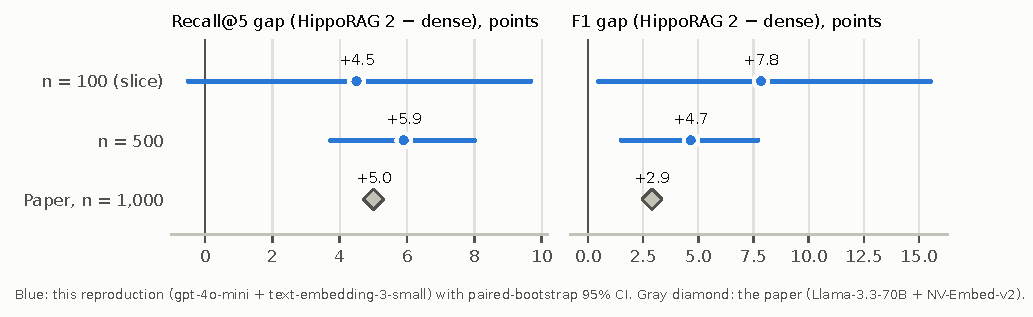
\includegraphics[width=\columnwidth]{figs/repro_gap.pdf}
\caption{HippoRAG 2 minus dense, in points, with paired-bootstrap 95\% intervals; the paper's gap for reference.}
\label{fig:repro}
\end{figure}
